
\documentclass[12pt,aspectratio=169]{beamer}

\input{style.tex}

\begin{document}

{\usebackgroundtemplate{\tikz\node[opacity=0.4,inner sep=0]{
\includegraphics[width=\paperwidth,height=\paperheight]{header}};}%
\begin{frame}[plain]
	\vspace{0.5cm}
	\title{\large \begin{spacing}{1.0}Fondamenti di Machine Learning\end{spacing}\vspace{0.25em}
		\normalsize \begin{spacing}{1.0}\textbf{Laurea Triennale in Ingegneria delle Comunicazioni}\end{spacing}\vspace{0.5em}}
	\subtitle{\Large \textbf{5: Classificazione (regressione logistica e Naive Bayes)}}
	\date{
		{
\includegraphics[scale=0.8]{Uniroma1}}
	}
	\author{
		\setlength{\tabcolsep}{2pt}
		\begin{tabular}{rl}
			\textbf{Lecturer}: & S. Scardapane \\
		\end{tabular}
	}\titlepage
\end{frame}
}

\part{1}

\section{Modelli per la classificazione}
\subsection{Formulazione del problema}

\begin{frame}{Classificazione}

	Passiamo ora ad affrontare più in dettaglio il problema della \myalert{classificazione}, nel quale la predizione $\hat{y}$ del modello può assumere solo un insieme finito di valori $\left\{1, \ldots, C\right\}$, corrispondenti alle \textit{classi} da predire (mutuamente esclusive). Ad esempio:
	%
	\begin{enumerate}
		\item Classificazione di immagini mediche (es., diagnostica).
		\item Predizione in un modello di generazione del testo (es., GPT).
		\item Classificazione di un cliente in un determinato segmento di mercato (es., possibile consumatore ricorrente).
		\item Predizione di quali clienti potrebbero lasciare l'azienda (\myalert{churn prediction}).
	\end{enumerate}

\end{frame}

\begin{frame}{Algoritmi per la classificazione}

	Abbiamo già visto come il $k$-NN possa essere usato per la classificazione (sostituendo la media con un voto di maggioranza), con tutti i limiti già menzionati. In questa lezione introduciamo invece due altri approcci:
	%
	\begin{itemize}
		\item Una estensione del least-squares a problemi di classificazione, la \myalert{regressione logistica} (o \myalert{logistic regression}).
		\item Come confronto, un semplice metodo probabilistico basato su una assunzione di indipendenza tra feature, il \myalert{Naive Bayes}.
	\end{itemize}

\end{frame}

\subsection{Least-squares regression}

\begin{frame}{Multi-output least-squares}

	Supponiamo di voler direttamente estendere il least-squares per predire la classe più probabile (\myalert{least-squares classification}). In questo caso, denotiamo come $\mathbf{y}$ il one-hot encoding della classe $y$ (es., se $y=2$ e $c=3$, $\mathbf{y}=[0 \;\; 1 \;\; 0]^\top$).

	Possiamo costruire un modello lineare con $c$ output come lo stack di $c$ diversi modelli unidimensionali:
	%
	\begin{equation}
		f(\mathbf{x}) = \begin{bmatrix} \mathbf{w}_1^\top \\ \vdots \\ \mathbf{w}_c^\top\end{bmatrix}\mathbf{x} + \begin{bmatrix} b_1 \\ \vdots \\ b_c \end{bmatrix} =
		\mathbf{W}\mathbf{x} + \mathbf{b}
	\end{equation}
	%
	dove $f(\mathbf{x}) \in \mathbb{R}^c$, $\mathbf{W} \in \mathbb{R}^{c \times d}$ e $\mathbf{b} \in \mathbb{R}^c$.

\end{frame}

\begin{frame}{Least squares classification}

	Possiamo allenare il modello minimizzando l'errore quadratico medio (in questo caso parliamo di \myalert{Brier score}); in fase di inferenza, la classe predetta diventa:
	%
	$$
		\text{Classe di } \vc{x} = \underset{k=1, \ldots, c}{\arg\max} \bigl\{ f_k(\vc{x}) \bigr\} \,.
	$$
	%
	Questo approccio è semplice da implementare ma ha diverse problematiche:
	%
	\begin{enumerate}
		\item Abbiamo perso una interpretazione probabilistica (i valori di $f$ possono essere negativi o maggiori di $1$).
		\item Per $c>2$, è possibile che una o più classi vengano mascherate.
	\end{enumerate}

\end{frame}

\begin{whiteframe}{Esempio di least squares classification}

	\begin{figure}
		\centering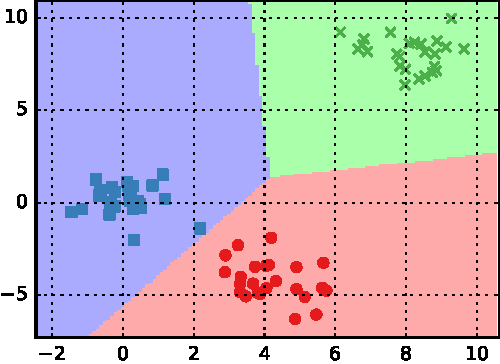
\includegraphics[width=8cm,keepaspectratio]{../scripts/ols_decision_boundaries_1.pdf} %
		\caption{Con $3$ classi perfettamente separabili, le \textbf{decision boundaries} trovate sono corrette.}
	\end{figure}

\end{whiteframe}

\begin{whiteframe}{Un esempio di class masking}

	\begin{figure}
		\centering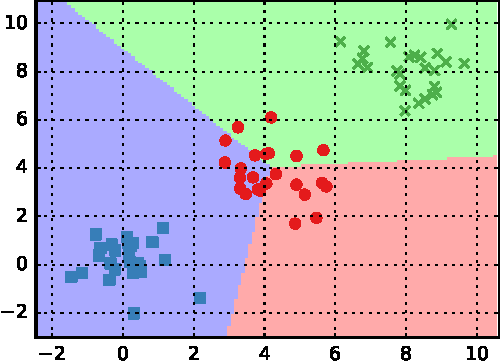
\includegraphics[width=8cm,keepaspectratio]{../scripts/ols_decision_boundaries_2.pdf} %
		\caption{In questo caso, nonostante le tre classi siano perfettamente separabili, una delle tre viene completamente mascherata dalle altre due.}
	\end{figure}

\end{whiteframe}

\subsection{Regressione logistica}

\begin{frame}{One-hot encoding}

	Riepilogando, possiamo rappresentare l'output in due modi: ad esempio, con tre classi:
	%
	\begin{itemize}
		\item $y = 1$, classe 1 (es., gatto).
		\item $y = 2$, classe 2 (es., cane).
		\item $y = 3$, classe 3 (es., altro).
	\end{itemize}
	%
	Oppure, con un one-hot encoding delle stesse classi:
	%
	\begin{equation}
		\text{Gatto: } \mathbf{y} = [1, 0, 0] \;\;\; \text{Cane: } \mathbf{y} = [0, 1, 0] \;\;\; \text{Altro: } \mathbf{y} = [0, 0, 1] \,.
	\end{equation}

\end{frame}

\begin{frame}{Interpretazione probabilistica}

	Vorremmo un modello che permetta di predire una \textit{distribuzione di probabilità} categorica sulle varie classi:
	%
	\begin{equation}
		p(\vc{y} \vert f(\vc{x})) = \prod_i f_i(\vc{x})^{y_i}
	\end{equation}
	%
	Per fare questo, l'output del modello deve rispettare queste due proprietà:
	%
	\begin{align}
		f_i(\vc{x}) \ge 0 \text{ (le probabilità sono positive) } \\ \sum_i f_i(\vc{x}) = 1 \text{ (le probabilità sommano ad 1) } \,.
	\end{align}

\end{frame}

\begin{frame}{La funzione softmax}

	La funzione \myalert{softmax} è definita come:
	%
	\begin{equation}
		\text{softmax}_i(\vc{a}) = \frac{\exp\left(a_i\right)}{\sum_j \exp\left(a_j\right)}
	\end{equation}
	%
	Un qualsiasi vettore $\text{softmax}(\vc{x})$ rispetta le due proprietà viste prima: positività (grazie al numeratore) e somma ad 1 (grazie al denominatore).

\end{frame}

\begin{whiteframe}{Visualizzazione della softmax}
	\begin{figure}
		\centering
		\subfloat[Softmax inputs (\myalert{logits})]{
			\centering
			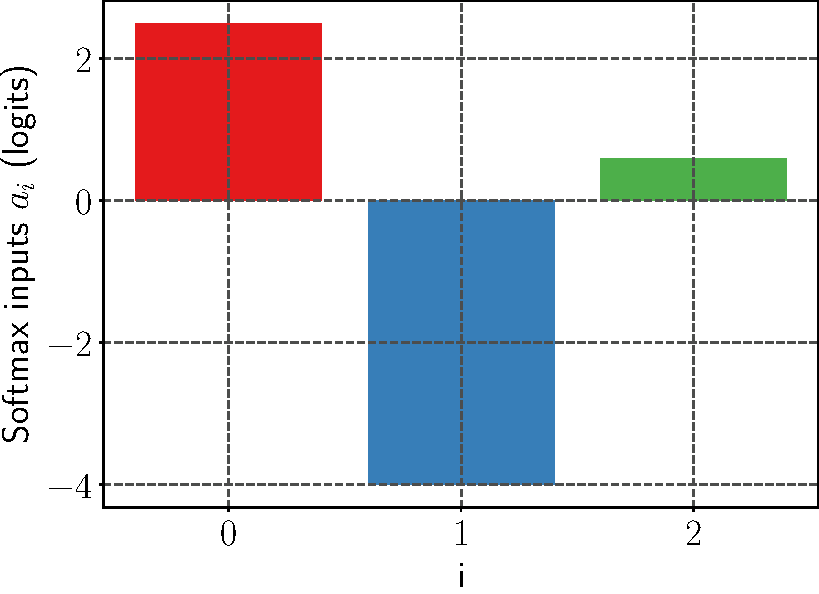
\includegraphics[width=0.45\textwidth]{../scripts/softmax_1}
		}
		\subfloat[Softmax outputs]{
			\centering
			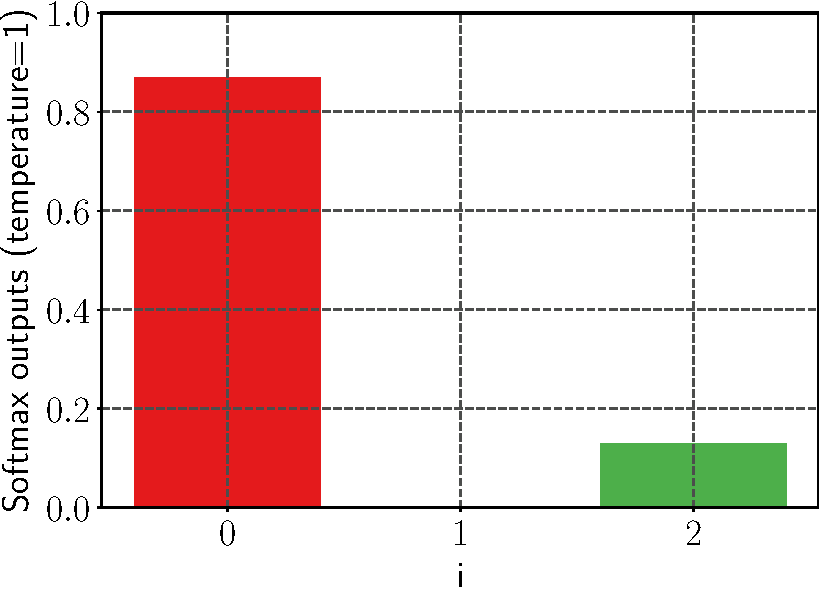
\includegraphics[width=0.45\textwidth]{../scripts/softmax_2}
		}
	\end{figure}
\end{whiteframe}

\begin{frame}{Modello lineare per la classificazione}

	Un modello lineare per la classificazione si ottiene combinando un classico modello lineare con la softmax:
	%
	\begin{equation}
		\stackunder{f(\vc{x})}{\sss (c)} = \text{softmax}(\stackunder{\vc{W}}{\sss (c,d)} \,\, \stackunder{\vc{x}}{\sss (d)})
	\end{equation}
	%
	I valori $\vc{W}\vc{x}$ vengono chiamati i \myalert{logits} del modello. Possiamo anche aggiungere esplicitamente i bias $\shape{\vc{b}}{(c)}$, ottenendo:
	%
	\begin{equation}
		f(\vc{x}) = \text{softmax}(\vc{W}\vc{x} + \vc{b}) \,.
	\end{equation}

\end{frame}

\begin{frame}{Cross-entropy}

	Per derivare una loss function applichiamo il principio di maximum likelihood, data la classe desiderata (one-hot encoded) $\vc{y}$ e le predizioni del modello $\hat{\vc{y}}$:
	%
	\begin{equation}
		L(\vc{y}, \hat{\vc{y}}) = - \log(p(\vc{y} \mid \hat{\vc{y}})) = - \sum_{i=1}^c y_i \log(\hat{y}_i)
	\end{equation}
	%
	Questa viene detta la \myalert{cross-entropy} loss.

\end{frame}

\begin{frame}{Log-likelihood loss}

	La cross-entropy loss ha una semplice interpretazione se ricordiamo che $\vc{y}$ è un vettore one-hot encoded. Denotando con $t$ l'indice della classe da predire, $t = \arg\max \vc{y}$, possiamo semplificare la CE notando che un solo termine è diverso da $0$:
	%
	\begin{equation}
		\text{CE}(\vc{y}, \hat{\vc{y}}) = - \log(\hat{y}_t) \,.
	\end{equation}
	%
	Quindi, minimizzare la CE porta semplicemente a massimizzare la probabilità predetta corrispondente alla classe desiderata.

\end{frame}

\begin{frame}{Regressione logistica}

	\begin{tcolorbox}
		Combinando il tutto, la \myalert{regressione logistica} è un modello lineare $f(\vc{x}) = \text{softmax}(\vc{W}\vc{x})$ allenato minimizzando la cross-entropy:
		%
		\begin{equation}
			\text{LR}(\vc{W}) = \frac{1}{n} \sum_{i=1}^n \text{CE}\left( \vc{y}_i, f(\vc{x}_i) \right) \,.
		\end{equation}
	\end{tcolorbox}
	%
	Non è più possibile risolvere questo problema in forma chiusa, ed è necessario ricorrere a metodi iterativi (es., discesa al gradiente). Un modello di questo tipo ha $dc$ parametri (o $dc + c$ considerando il bias).

\end{frame}

\subsection{Classificazione binaria}

\begin{frame}{Classificazione binaria}

	La \myalert{binary classification}, $c=2$, permette una serie di semplificazioni. In effetti, possiamo predire un unico valore $f(\vc{x}) \in \left[0, 1\right]$:
	%
	\begin{align}
		f(\vc{x})     & \;\;\; \text{ probabilità della classe 1 } \,, \\
		1 - f(\vc{x}) & \;\;\; \text{ probabilità della classe 2 } \,.
	\end{align}
	%
	In questo caso la softmax diventa la funzione \myalert{sigmoide}:
	%
	\begin{tcolorbox}
		La sigmoide (o funzione sigmoidea) $\sigma(s) \in \left[0, 1 \right]$ è definita come:
		%
		\begin{equation}
			\sigma(s) = \frac{1}{1 + \exp(-s)} \,.
		\end{equation}
	\end{tcolorbox}

\end{frame}

\begin{whiteframe}{Visualizzazione}

	\begin{figure}
		\centering
		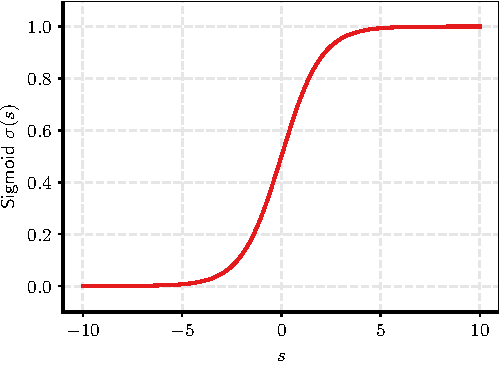
\includegraphics[width=0.6\columnwidth]{../scripts/sigmoid.pdf}
		\vspace{-0.5em}\caption{Visualizzazione della funzione sigmoidea. Si noti come $0$ e $1$ vengono raggiunti solo asintoticamente.}
	\end{figure}

\end{whiteframe}

\begin{frame}{Regressione logistica binaria}

	Combinando i due otteniamo un modello di regressione logistica valido solo nel caso binario:
	%
	\begin{equation}
		\text{BIN-LR}(\vc{w}) = \frac{1}{n} \sum_{i=1}^n \Bigl[ -\underbrace{y_i\log\left(\sigma(\vc{w}^\top\vc{x}_i)\right)}_{\text{Classe 1}} - \underbrace{(1-y_i)\log\left( 1 - \sigma(\vc{w}^\top\vc{x}_i)\right)}_{\text{Classe 2}} \Bigr]
	\end{equation}
	%
	In questo caso, la classe predetta dal modello diventa:
	%
	\begin{equation}
		\text{classe} = \begin{cases}
			1 & \text{ se } \sigma(\vc{w}^\top\vc{x}) > 0.5 \,, \\
			0 & \text{ altrimenti } \,.
		\end{cases}
	\end{equation}

\end{frame}

\begin{frame}{Gradiente della regressione logistica}

	Consideriamo il gradiente della sigmoide:
	%
	\begin{equation}
		\sigma'(s) = \sigma(s)(1 - \sigma(s)) \,.
	\end{equation}
	%
	Inserendolo nel calcolo del gradiente della regressione logistica binaria otteniamo:
	%
	\begin{equation}
		\nabla \text{BIN-LR}(\vc{w}) = \frac{1}{n} \sum_{i=1}^n (\sigma(\vc{w}^\top\vc{x}_i) - y_i)\vc{x}_i \,.
	\end{equation}
	%
	Si noti la similarità con il caso della regressione.

\end{frame}

\begin{frame}{Generalized linear models}

	In effetti, possiamo riscrivere il modello come:
	%
	\begin{equation}
		\underbrace{\mathbf{w}^\top \mathbf{x}+b}_{\text{logits}}=\underbrace{\log\left(\frac{f(\vc{x})}{1-f(\vc{x})}\right)}_{\sigma^{-1}(f(\vc{x}))}
	\end{equation}
	%
	Questo chiarisce perché ci riferiamo alla regressione logistica come ad un modello lineare: è equivalente ad un modello lineare allenato su una transformazione non-lineare dell'output. Questa classe di modelli viene detta \myalert{generalized linear models}.

\end{frame}

\subsection{Naive Bayes}

\begin{frame}{Naive Bayes (introduzione)}

	Concludiamo con una semplice baseline per la classificazione, chiamata \myalert{Naive Bayes}.
	Ricordiamo il teorema di Bayes:
	%
	\begin{equation}
		p(y \mid \mathbf{x}) = \frac{p(\mathbf{x} \mid y)p(y)}{p(\mathbf{x})} \,.
	\end{equation}
	%
	Si noti come $p(y)$ (detta la \myalert{prior distribution} sulle classi) è relativamente semplice da stimare con metodi frequentisti. Inoltre, nel caso ci interessi solo il massimo di $p(y \mid \mathbf{x})$, possiamo ignorare il denominatore (costante per ogni classe).

\end{frame}

\begin{frame}[fragile]{Approssimazione del Naive Bayes}

	Per rendere il problema trattabile, l'assunzione di base del \myalert{Naive Bayes} è che ogni feature è indipendente \myalert{data la classe}:\blfootnote{Errore comune: questo non comporta che le feature siano indipendenti \textit{a prescindere}. In pratica, questa assunzione raramente è valida, ma il classificatore funziona sorprendentemente bene in molte applicazioni.}
	%
	\begin{equation}
		p(\mathbf{x} \mid y) = \prod_{i=1}^d p(x_i \mid y)
	\end{equation}
	%
	Sotto questa assunzione, ogni termine $p(x_i \mid y)$ è una semplice distribuzione univariata che può essere stimata a partire dai dati.

\end{frame}

\begin{frame}{Stimare i parametri del Naive Bayes}

	Ad esempio, supponiamo che $x_i$ sia una feature categorica con $n_i$ classi. In questo caso, $p(x_i \mid y)$ diventa una distribuzione categorica, e:
	%
	\begin{equation}
		p(x_i = j \mid y) = \frac{\lvert \left\{ (\mathbf{x}, y^\prime) \in \mathcal{S} \mid x_i = j \text{ e } y^\prime = y \right\}\rvert}{\lvert \left\{ (\mathbf{x}, y^\prime) \in \mathcal{S} \mid y^\prime = y \right\}\rvert}
	\end{equation}
	%
	dove $n$ è la dimensione del dataset. Questo non richiede altro che contare in maniera opportuna gli elementi del dataset.

	Nel caso di una feature continua, possiamo stimare media e varianza di una Gaussiana univariata (condizionale alla classe).

\end{frame}

\begin{frame}{Il problema della probabilità zero}

	Cosa succede se un determinato valore $x_i = j$ non compare mai nel training set insieme ad una classe $y$? La probabilità empirica diventa zero:
	%
	\begin{equation}
		p(x_i = j \mid y) = 0 \implies p(\mathbf{x} \mid y) = 0
	\end{equation}
	%
	L'intera probabilità predetta si annulla, indipendentemente dai valori delle altre feature. Per evitare questo, si applica una tecnica detta \myalert{Laplace smoothing} (o additive smoothing), aggiungendo un termine $\alpha > 0$ (spesso $\alpha = 1$) ai conteggi:
	%
	\begin{equation}
		p(x_i = j \mid y) = \frac{\lvert \left\{ (\mathbf{x}, y^\prime) \in \mathcal{S} \mid x_i = j \text{ e } y^\prime = y \right\}\rvert + \alpha}{\lvert \left\{ (\mathbf{x}, y^\prime) \in \mathcal{S} \mid y^\prime = y \right\}\rvert + \alpha n_i}
	\end{equation}
	%
	In questo modo nessuna probabilità è mai esattamente nulla.

\end{frame}

\begin{frame}{Classificazione con Naive Bayes}

	Riscrivendo nel dominio logaritmico, scegliamo quindi la classe che massimizza la quantità:
	%
	\begin{equation}
		y^* = \underset{y}{\arg\max} \left\{ \log p(y) + \sum_i \log p(x_i \mid y) \right\}
	\end{equation}
	%
	Si può estendere Naive Bayes al caso di regressione trasformando l'output $y$ con un binning in un numero predeterminato di intervalli (ma è meno comune).

\end{frame}

\begin{whiteframe}{Visualizzare Naive Bayes}

	\begin{figure}
		\centering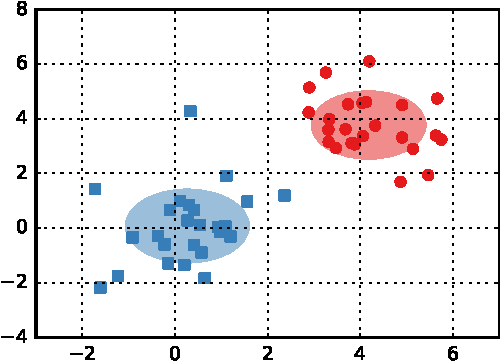
\includegraphics[width=8cm,keepaspectratio]{../scripts/naive_bayes.pdf} %
		\caption{Esempio di Naive Bayes su un semplice dataset 2D con due distribuzioni Gaussiane univariate.}
	\end{figure}

\end{whiteframe}

\end{document}
